\documentclass[11pt]{extarticle}
\usepackage{manualdoprofessor}
\usepackage{fichatecnica}
\usepackage{lipsum,media9}
\usepackage[justification=raggedright]{caption}
\usepackage[one]{bncc}
\usepackage[acorde]{../edlab}
\usepackage{marginnote}
\usepackage{pdfpages}
%\usepackage[printwatermark]{xwatermark}
%\newwatermark[pagex=2]{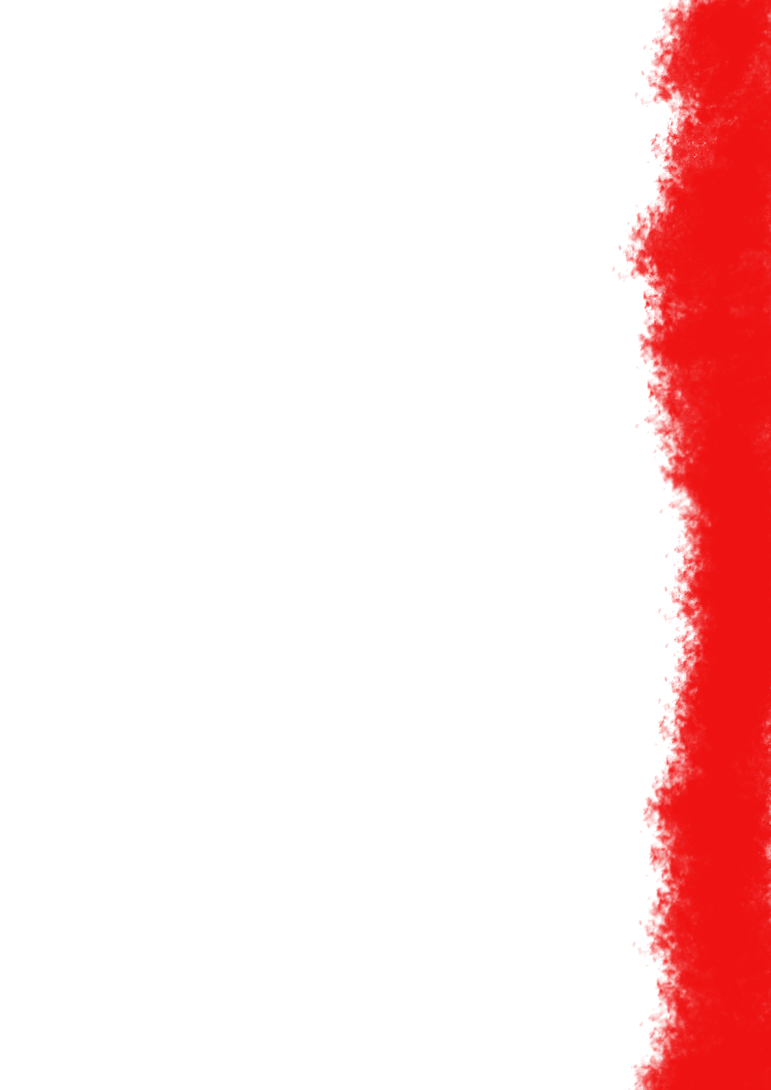
\includegraphics[scale=3.3]{watermarks/test-a.png}}	% página específica
%\newwatermark[oddpages]{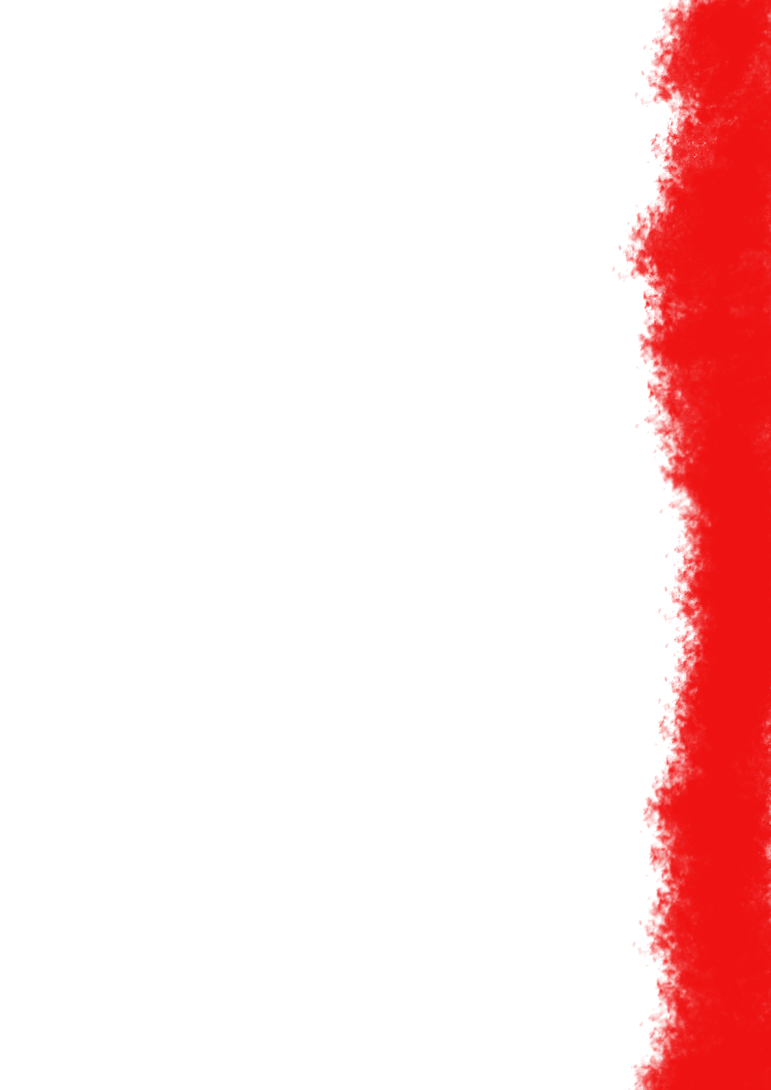
\includegraphics{watermarks/test-a.png}}			% páginas ímpars
%\newwatermark[evenpages]{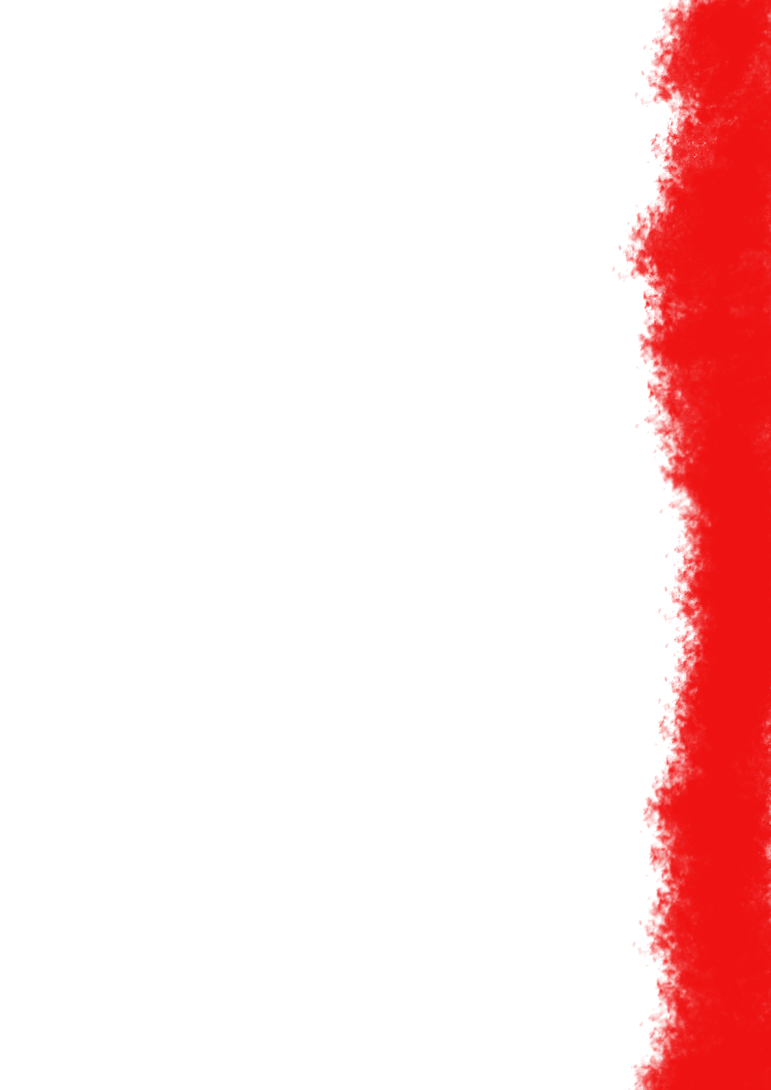
\includegraphics{watermarks/test-a.png}}			% págimas pares
%\newwatermark[allpages]{\includegraphics[scale=1]{watermarks/001.png}}

%\pagecolor{cyan!0!magenta!10!yellow!28!black!28!}

\newcommand{\AutorLivro}{Eloar Guazzelli}
\newcommand{\TituloLivro}{Mr. Pillow é um fantasma!}
\newcommand{\Genero}{Conto; crônica; novela}
%\newcommand{\imagemCapa}{./pdf/capa.jpg}
\newcommand{\issnppub}{XXX-XX-XXXXX-XX-X}
\newcommand{\issnepub}{XXX-XX-XXXXX-XX-X}
% \newcommand{\fichacatalografica}{PNLD0001-00.png}
\newcommand{\colaborador}{Renier Silva}

\begin{document}

\title{\TituloLivro}
\author{\AutorLivro}
\def\authornotes{\colaborador}

\date{}
\maketitle

%\begin{abstract}\addcontentsline{toc}{section}{Carta ao professor}
%\pagebreak

\tableofcontents




\begin{abstract}

Caros professores e professoras, 

esperamos, com este material,
auxiliá-los no trabalho com o \textbf{Ensino Fundamental \textsc{ii}} em sala de aula.
\textit{Mr. Pillow é um fantasma!}, de Eloar Guazzelli, é um livro singular
por vários motivos e possibilita atividades didáticas interessantíssimas,
como vocês acompanharão a seguir.

Uma dos pontos mais curiosos deste livro é justamente a sua escrita.
Trabalhado aqui com alunos do \textbf{Ensino Fundamental \textsc{ii}},
o autor opta por utilizar elementos de caligrafia, ortografia e sintaxe 
próprios dos pré-adolescentes nesta fase do desenvolvimento escolar.
Portanto, um dos aspectos que parecem interessantes de ser tratados durante
todas as atividades do livro é o mundo da \textbf{escrita}, sua regras
e convenções.

Além desse, outro enfoque que merece atenção é o universo mítico presente
em todas as culturas. Como será visto na narrativa, o fantasma britânico,
com suas características próprias que o adjetivo lhe atribui, conhece
outros, particulares ao novo lugar onde se encontra --- a Floresta Amazônica.
Este movimento oferece uma boa oportunidade de se estudar, com os alunos, 
o que a \textsc{bncc} propõe como ``\textbf{concepções de mundo}, natureza, ser humano, 
divindades, vida e morte em diferentes mitos de criação''. Assim, 
noções primárias de \textbf{multiculturalismo} poderão ser bem aproveitadas
nesta etapa.

Por último, não deixemos de levar em conta o ensejo de estudar o momento
histórico do \textbf{ciclo da borracha}, contexto histórico de fundo 
na narrativa. Menos que uma paisagem inerte, porém, são os interesses
e desenvolvimentos deste período que ocasionaram nas movimentações
ocorridas na narrativa: o fantasma da Inglaterra vai parar na Amazônia
porque, em vida, foi um grande investidor nos negócios da borracha do Brasil. 

Esperamos, por fim, professor ou professora, que este material sirva como um guia 
para seu trabalho em sala de aula. Já contamos, no entanto, com as adaptações
que surgirão organicamente na recepção do mesmo por vocês, que possuem 
trajetórias e escolhas didáticas específicas, bem como no contato com os 
alunos, que tanto têm a oferecer para o enriquecimento da experiência didática. 

Boa aula!

\end{abstract}
\section{Sobre o livro}

%550 caracteres
\paragraph{O livro} \textit{Mr. Pillow é um fantasma!} apresenta a narrativa um fantasma tipicamente inglês 
que mora num castelo da Inglaterra. Devido a sua condição de fantasma, ele deve acompanhar
os objetos que eram seus durante a vida. Por isso, quando decidem realocar as pedras do castelo para 
a Floresta Amazônica, ele vai junto. Esta mudança de territórios, tão distantes geograficamente
e em costumes, se deve ao fato de que Mr. Pillow, em vida, juntou sua fortuna com a exploração de borracha
nessa região.

Ao chegar na nova paisagem, o fantasma de Mr. Pillow conhece os seres míticos que habitam a região da Amazônia
brasileira. Ele não se adapta muito bem ao novo contexto, porém, e finda a narrativa de volta à sua
terra natal, graças a um ``serviço de transferências'' do mundo dos fantasmas. 

Aspecto importante deste livro é que ele é escrito com ortografia, caligrafia e sintaxe 
particulares a uma criança ou pré-adolescente em estágio de desenvolvimento da 
escrita. À primeira leitura, inclusive, tal procedimento deverá causar estranhamento 
e dificuldade aos leitores acostumados com a escrita padrão. Por outro lado,
para os alunos, pode funcionar como fator de identificação e tornar a leitura
ainda mais prazerosa, e instrutiva, caso o professor ou professora aproveite o
ensejo para comentar a padronização da linguagem escrita. 



\section{Sobre o autor}

\paragraph{Eloar Guazzelli}

%inserir foto do autor à margem 

Eloar Guazzelli Filho, ou apenas \textbf{Guazzelli}, nasceu em Vacaria, Rio Grande do Sul, em 1962. 
Torce para o Internacional de Porto Alegre, gosta de jogar futebol nas areias de Florianópolis, onde passa o verão, mas é ruim de bola. Artista plástico, quadrinista, roteirista e diretor de arte para animação, é formado pelo Instituto de Artes da Universidade Federal do Rio Grande do Sul (\textsc{ufrgs}) e mestre pela Escola de Comunicação e Artes da Universidade de São Paulo (\textsc{eca--usp}). Recebeu inúmeras premiações em todo o Brasil e participou de exposições em mais de quinze países.

Desenhista há 29 anos, consagrou-se no universo das histórias em quadrinhos e também faz animações para o cinema. 
Já ilustrou mais de 60 livros para crianças, entre eles, \textit{Maluquices Musicais} e \textit{Futebolíada} com o parceiro José Santos, \textit{Grande sertão: veredas}, de Guimarães Rosa, lançada em 2021,
\textit{Zoo zoado}, de Fabrício Corsaletti, de 2014, \textit{O segredo} e \textit{Histórias de mistério}, de Lygia Fagundes Telles, de 2012 e 2011, respectivamente, e \textit{O menino que caiu do céu}, de Lucy Coats, de 2009.

Além de ilustrador, é um grande leitor, sobretudo, dos clássicos da literatura mundial.
Dentre as obras que escreveu, estão \textit{A divina jogada} e \textit{Apocalipse nau}, de 2015, e \textit{Mr. Pillow é um fantasma!}, aqui presente.


\section{Sobre o gênero}

\paragraph{O gênero} O gênero deste livro é a \textit{conto; crônica; novela}. 

%596 caracteres
\paragraph{Descrição} O que define um gênero narrativo é o fato de, não importa
qual seja sua forma, eles \textit{contarem uma história}.
As especificidades do \textit{como} esta história será contada é que
qualificaram os tipos de gênero narrativo, que podem ser: conto, crônica, novela,
epopeia, romance ou fábula. 

Toda narrativa possui, necessariamente, um narrador, uma personagem, um enredo,
um tempo e um espaço. O narrador, ou narradora, pode ser onisciente, literalmente
\textit{que tudo sabe}, observador ou personagem --- categorias que não são autoexclusivas.
O discurso elaborado por este narrador ou narradora pode ser direto, indireto ou indireto livre 
--- ou seja, ele ou ela pode aparecer mais diretamente ou mais indiretamente; no último caso,
sua voz se mistura à das personagens da história.

O narrador \textbf{não é necessariamente} a voz do autor. É errada a afirmação
de que o autor fala através do narrador de uma história. É bastante comum,
há algum tempo na história literária, sobretudo desde os pré-modernistas, que 
o narrador represente justamente o contrário do que pensa o autor. Neste caso, 
utiliza-se elementos como a \textbf{ironia} para sugerir que o autor \textit{não é confiável}.

Já as persponagens variam quanto a sua \textbf{profundidade}. Há personagens planas, ou
personagens-tipo, e personagens redondas, ou complexas. Personagens planas
são facilmente repetíveis pois se amparam em lugares-comuns da cultura, como
o vilão, o herói, a vítima, o palhaço, tudo isso com marcações de gênero e espécie ---
o herói tradicionalmente é um homem, a vítima, uma mulher, e o vilão, uma figura que 
se afasta da humanidade por alguma razão, às vezes sobrenatural. 
Personagens redondos, por outro lado, estão mais próximos das \textit{pessoas reais}.
Uma personagem complexa pode ser, em um dado momento da narrativa, vilã, e em 
outro, heroina. É importante notar como as visões de mundo, um traço cultural e 
portanto relativo, influenciam na caracterização das personagens, planas 
ou redondas, de uma história.

O tempo de uma narrativa pode ser cronológico ou psicológico.
No tempo cronológico, o enredo segue a ordem ``normal'' dos acontecimentos,
aquela marcada pelo relógio e pelo calendário. Os acontecimentos vêm um após o 
outro e se delimita muito bem \textit{passado}, \textit{presente} e \textit{futuro}.
Já no tempo psicológico, segue-se uma ordem \textit{subjetiva} dos acontecimentos, 
e portanto, \textit{não linear}, já que a influência emocional e psíquica 
da subjetividade afeta a racionalidade do tempo cronológico. 

O espaço, por fim, é o lugar onde se passa a narrativa. Dependendo do caso, 
ele pode funcionar mais como um plano de fundo, sem muita interferência
no enredo, ou mais ativamente, aproximando-se das características das personagens
e influenciando no desenrolar da trama. 

O último aspecto de um gênero narrativo que podemos abordar é sua 
\textit{extensão}. Dentre os elementos que distinguem um subgênero 
de outro é o tamanho da história: uma crônica e um conto são \textit{necessariamente}
curtos, ao passo que uma epopeia e um romance, são longos. Uma novela
está no ponto intermediário entre um romance e um conto.
Ainda poderíamos falar dos registros de cada subgênero: 
a epopeia é originalmente um subgênero \textit{oral}, versificado, e metrificado,
já o romance é tradicionalmente \textit{escrito} em prosa. 
Desde meados do século \textsc{xviii}, no entanto, o estabelecimento
dos gêneros e subgêneros narrativos tornam-se cada vez menos rígido,
com as características cada vez mais fluidas e intercomunicativas.

Como o presente livro se trata de uma narrativa \textit{curta},
finalizamos com as palavras de Luiza Vilma Pires a respeito do
subgênero:

\begin{quote}
sob o nome de narrativa curta, estão situadas obras que apresentam uma trama 
um pouco mais complexa, que ocorre em diversos espaços e em uma temporalidade 
que pode ser de vários dias, semanas ou meses. Entretanto a função das ilustrações 
continua as mesmas, são complementares à história e contribuem para sua compreensão. 
Os temas relacionam-se a vivência infantis (brincadeiras, passeios, pequenas aventuras), 
a aspectos ligados à interioridade das personagens (busca de identidade, insegurança, 
medos) ou a relações interpessoais (desentendimentos familiares, entre amigos, solidariedade).\footnote{“Narrativas infantis”, de Luiza Vilma Pires Vale. In \textsc{saraiva}, J. A. (Org.) \textit{Literatura e alfabetização: do plano do choro ao plano da ação}. Porto Alegre: Artmed, 2001.} 
\end{quote}


\section{Atividades}

\subsection{Pré-leitura}

\paragraph{Atividade 1}

\BNCC{EF05ER02}
\BNCC{EF05ER03}
\BNCC{EF05ER05}
\BNCC{EF05HI01}

\paragraph{Tema} Os diferentes espaços geográficos.

\paragraph{Conteúdo} Sensibilização a respeito das diferentes mitologias
e crenças conforme as culturas.

\paragraph{Justificativa} Um tema que percorre o enredo de \textit{Mr. Pillow é um fantasma!}
ainda que não de forma explícita é a concomitância de diferentes narrativas mitológicas.
Graças ao deslocamento geográfico do fantasma Mr. Pillow, da Inglaterra à Amazônia brasileira, 
o leitor se depara com diferentes figuras do imaginário de cada região. 
Este pode ser um ótimo ensejo para se tratar, de forma adequada à série,
alguns aspectos do multiculturalismo. 

\Image{Típico castelo britânico assombrado.(CC-BY-2.0)}{PNLD2023-028-01.jpg}
\Image{Interior da Floresta Amazônica.(CC-BY-2.0)}{PNLD2023-028-02.jpg}

\paragraph{Metodologia} Para iniciar a conversa com os alunos,
o professor pode fazer as seguintes perguntas:

\begin{itemize}
\item Quais as diferenças mais marcantes entre os dois espaços?
\item Qual dos dois é mais ``fantasmagórico''?
\item Qual lhes dá mais medo?
\end{itemize}

Às vezes, uma mesma figura ou um mesmo mito pode aparecer em diferentes culturas.
Este é o caso da \textbf{Iara}, dos povos indígenas amazônicos. 

Após a discussão, peça aos alunos que \textbf{realizem uma pesquisa acerca das mitologias} 
brasileira e inglesa --- ou europeia, mais vastamente. 

\Image{A sereia é uma criatura mitológica presente na cultura ibérica que mantém semelhanças 
com a Iara amazônica.(CC-BY-2.0)}{PNLD2023-028-05.jpg}

\paragraph{Tempo estimado} Duas aulas de cinquenta minutos.


\section{Leitura}

\paragraph{Atividade 1} 

\paragraph{Tema} Leitura oral e padronização da escrita.

\paragraph{Conteúdo} Prática de leitura alternada entre os estudantes 
e regras ortográficas e gramaticais como o \textbf{uso do acento circunflexo no 
verbo \textit{ter}} e o \textbf{uso da vírgula}.

\paragraph{Justificativa} O presente livro apresenta uma cara oportunidade 
de se trabalhar aspectos da gramatica normativa em sala de aula com os alunos
já que sua escrita não segue estritamente a norma padrão.
Desde sua fonte, que imita uma escrita à mão de uma criança na faixa etária
dos estudantes, até à própria sintaxe e o uso vocabular. Alguns pequenos erros,
comuns à esta fase do desenvolvimento da linguagem, são encontrados,
e devem ser aproveitados como ensejo didático. 

\paragraph{Metodologia} O professor ou a professora deve realizar a leitura
em sala de aula com os alunos. Intercale a leitura de modo que todos tenham a 
oportunidade de ler, sempre em voz alta. 

Quando lerem as primeiras frases, chame a atenção à estrutura da linguagem.
\textbf{É inusitado para os alunos um livro escrito daquele jeito?}
Conforme a leitura decorra, faça uma pausa na ocasião das seguintes frases:

\begin{itemize}
	\item ``Só os fantasmas \textit{tem} ideia de como isso pode ser bom.''
	\item ``Ah tá, pode fica esperando pensava Mr. Pillow.''
\end{itemize}


\Image{Excerto das primeiras páginas do livro.}{PNLD2023-028-06.jpg}
\Image{Excerto das primeiras páginas do livro.}{PNLD2023-028-07.jpg}


No caso da primeira frase, indique que há um erro na grafia da palavra
\textit{tem}, verbo ter conjugado na terceira pessoa do plural 
no modo indicativo do tempo presente. Escreva na lousa a conjugação
completa de tal verbo, a saber:

\begin{verse}
Eu tenho\\
Tu tens\\
Você \textbf{tem}\\
Ele/ ela/ a gente \textbf{tem}\\
Nós temos\\
Vós tendes\\
Vocês \textbf{têm}\\
Eles/ elas \textbf{têm}\\
\end{verse}

Em resumo, a regra gramatical que precisa ser fixada aqui é que
\textbf{o acento circunflexo é utilizado em alguns verbos para
indicar que se trata do plural e não do singular}. Ele
não tem nenhuma função fonética; ou seja, \textit{tem} e \textit{têm}
são pronunciados da mesma forma.
Deste modo, diz-se: ``Mr. Pillow \textbf{tem} ideia de como isso pode ser bom.''
Mas: ``Os fantasmas \textbf{têm} ideia de como isso pode ser bom.''

Aproveite o ensejo para trabalhar a diferença entre os verbos \textit{vir}
e \textit{ver}, onde o acento circunflexo também tem uma função 
diferenciadora, e não fonética. 
Na terceira pessoa do plural do verbo \textit{vir}, dizemos: ``Eles \textbf{vêm}.''
Na terceira do singular: ``Ele \textbf{vem}.'' A regra é a mesma do verbo \textit{ter}. 
Já quanto ao verbo \textit{ver}, o acento é usado em outro contexto.
A terceira pessoa do plural, no modo indicativo presente, dos dois verbos
é \textbf{pronunciada} da mesma forma: / \textit{vem}/. Na escrita, porém, há diferenças.
No caso do verbo \textit{vir}, já vimos que teremos \textbf{vêm}, já para
o verbo \textit{ver}, teremos \textbf{veem}. 

Aproveite para apresentar toda a conjugação dos dois verbos no presente do indicativo,
onde tais características aparecem:

\begin{verse}
Eu venho\\
Tu vens\\
Você \textbf{vem}\\
Ele/ ela/ a gente \textbf{vem}\\
Nós vimos\\
Vós vindes\\
Vocês \textbf{vêm}\\
Eles/ elas \textbf{vêm}\\
\end{verse}

\begin{verse}
Eu vejo\\
Tu vês\\
Você vê\\
Ele/ ela/ a gente vê\\
Nós vemos\\
Vós vedes\\
Vocês \textbf{veem}\\
Eles/ elas \textbf{veem}\\
\end{verse}

Resolvida a questão do uso do acento circunflexo com caráter diferenciador e não fonético
--- o professor ou professora deve se sentir à vontade para trabalhar da forma que lhe convir,
apresentando mais exemplos ou mesmo distribuindo à turma uma lista de exercícios que tratem do tema ---
podemos partir para \textbf{o uso da vírgula}.

São muitas as regras a respeito do uso da  vírgula em língua portuguesa. 
Muitas delas serão estudadas no decorrer do \textbf{Ensino Fundamental \textsc{ii}} e outras,
somente no \textbf{Ensino Médio}. 
Sugerimos, portanto, que o professor se detenha no exemplo retirado do livro. 

Escreva a frase na lousa. ``Ah tá, pode ficar esperando pensava Mr. Pillow.''
Pergunte, então, aos alunos, se eles sentem que há algo de errado. Leia em voz
alta e então peça que repitam. Faça questão de \textbf{não realizar nenhuma pausa}
entre as palavras \textit{esperando} e \textit{pensava}.
Repita o exercício até que fique claro o problema da \textbf{falta de vírgula} na frase,
e então explique que, neste caso, a vírgula \textbf{intercala duas orações}. 
Ou seja, nesta frase há duas orações:

\begin{itemize}
	\item Mr. Pillow pensava
	\item Ah tá, pode ficar esperando
\end{itemize}

Uma solução para alternar o uso da vírgula seria usar \textbf{dois pontos} e \textbf{aspas} ---
usados quando queremos indicar um discurso diretamente. 
Neste caso, teríamos: \textit{Mr. Pillow pensava\textbf{:} \textbf{``}Ah tá, pode ficar esperando!\textbf{''}}
Já com a vírgula, a frase fica escrita corretamente assim: \textit{Ah tá, pode ficar esperando\textbf{,}
pensava Mr. Pillow.}

Do mesmo modo que no estudo do uso do acento circunflexo, o professor ou professora pode estender
a atividade com a aplicação de exercícios para tratar do tema da vírgula.
Não deixe de levar em consideração, no entanto, a série da turma para não haver
decalagem de conteúdo. 

\paragraph{Tempo estimado} Quatro aulas de cinquenta minutos.

\paragraph{Atividade 2}

Ainda no decorrer da leitura, depois de trabalhadas as questões gramaticais, 
chame a atenção para pontos importantes da narrativa como as diferenças entre 
o fantasma britânico e os seres amazônicos. Verifique com os alunos uma diferença
fundamental entre ambos: o primeiro vive no \textbf{ambiente urbano}, em um castelo, uma 
obra arquitetônica construída por seres humanos, e os outros, na \textbf{ambiente rural},
na floresta, um espaço onde a interferência humana não se dá da mesma forma que 
no primeiro caso. 

Quais as reverberações que estas características podem ter na vida das pessoas e, 
consequentemente, nos elementos das histórias que elas constroem? 
Faça perguntas como esta ligadas ao tema e promova uma discussão entre a turma.  


\section{Pós-leitura}

\BNCC{EF68AR33}
\BNCC{EF69AR34}
\BNCC{EF69LP44}

\paragraph{Atividade 1} 

\paragraph{Tema} O ciclo da borracha na região amazônica no século \textsc{xx}.

\paragraph{Conteúdo}Pesquisa e discussão acerca do contexto histórico e social 
do ciclo da borracha amazônico no século \textsc{xx}.

\paragraph{Justificativa} Toda obra cultural e artística está ancorada em valores e 
visões de mundo que remetem a um determinado período histórico. 
É essencial que alunos e alunas sejam capazes de perceber como 
dados da realidade ``exterior'' à obra (os fatos da história) estão
presentes na construção e no desenvolvimento da narrativa. No caso 
de \textit{Mr. Pillow é um fantasma!}, o momento histórico que se 
destaca é \textbf{ciclo da borracha} na região amazônica em meados
do século \textsc{xx}.

\paragraph{Metodologia} Após a leitura do livro, peça à turma que se divida em grupos.
Eles realização uma pesquisa seguida de um seminário acerca do tema: \textbf{ciclo da borracha na Amazônia}.
O professor ou professora pode indicar aos alunos e alunos os materiais 
audiovisuais e escritos que deixamos na \textbf{Sugestão de referências complementares}.

\Image{Extração de borracha na Amazônia.(CC-BY-2.0)}{PNLD2023-028-03.jpg}

Como terá se observado na pesquisa feita acerca da Fordlândia, um dos motivos
que levaram à eclosão de revoltas dos trabalhadores foi a \textbf{diferença cultural}
entre os hábitos locais dos trabalhadores rurais brasileiros e os hábitos urbanos 
dos patrões estadunidenses. A alimentação, um relevante aspecto cultural,
foi algo que minou a relação entre empregados e patrões: eram servidos hambúrgueres, 
prato tradicional das grandes cidades dos Estados Unidos, a uma população acostumada 
com pratos nutritivamente, mas não só, diversos deste. Outros pontos como a disciplina
de trabalho causaram problemas de adaptação que, somados a outros fatores de 
ordem econômica e política, levaram ao fim o projeto.

\Image{Caixa d'água e escritório central de Fordlândia. Mesmo na arquitetura percebem-se elementos 
incomuns em relação à tradição rural da região amazônica.(CC BY-SA 3.0)}{PNLD2023-028-08.jpg}

A partir desta explanação, o professor ou a professora pode elaborar a seguinte
discussão com a turma, tendo o enredo do livro como objeto:
\begin{itemize}
\item Por que o fantasma inglês não se adapta ao Brasil?
\end{itemize}

\paragraph{Atividade 1.2}

Para finalizar o trabalho com o livro, os alunos deverão \textbf{produzir uma história}
de cunho fantástico tal qual \textit{Mr. Pillow é um fantasma!} tendo como espaço
a Fordlândia. Elementos visuais descobertos com a pesquisa devem ser trabalhados, 
como a existência de obras arquitetônicas de origem estrangeira abandonadas no meio 
da floresta.
Instigue a imaginação dos alunos e alunas com a seguinte provocação: \textbf{como seria
uma fábrica fantasma no meio da Floresta Amazônica?}

Ao fim da atividade, todos podem compartilhar suas criações entre si
numa roda de leitura. 

\paragraph{Tempo estimado} Quatro aulas de cinquenta minutos.



\section{Sugestões de referências complementares}

\subsection{Filmes e documentários} 
\begin{itemize}

\item \textsc{educação}, Ministério da. \textit{A história da borracha amazônica}. Disponível em: \url{https://www.youtube.com/watch?v=_qoIDCSBNsI}. Último acesso em 17 de dezembro de 2021.

O documentário mostra como era a vida nos seringais, os conflitos com os povos indígenas e as 
queimadas do Acre, além de contar a história do líder ambientalista Chico Mendes e a reserva extrativista.

\end{itemize}

\subsection{Artigos}

\begin{itemize}
	\item ``Fordlândia: breve relato da presença americana na Amazônia''. Disponível em : \url{https://periodicos.saude.sp.gov.br/index.php/cadernos/article/view/35751}. Último acesso em 17 de dezembro de 2021.

	Destinada a ser a primeira “cidade empresa” edificada na Amazônia, oferecia a seus habitantes: hospital, escola, água encanada, luz elétrica, moradia, lazer e emprego. A baixa produtividade, o fim da Segunda Guerra Mundial com consequente queda na demanda mundial por borracha, e a produção de borracha sintética levaram à retirada dos americanos da região do Tapajós em 1945. O governo federal adquiriu as benfeitorias e as plantações de seringueiras, porém não impediu a degradação de Fordlândia que viu seu patrimônio material ser dilapidado, ficando prédios em ruínas e lembranças de moradores remanescentes do tempo do fastígio da borracha. 


	\item ``Borracha, nordestino e floresta: A economia e a sociedade amazônica nos dois ciclos gomíferos''. Disponível em: \url{https://periodicos.ufpa.br/index.php/cepec/article/view/6773/0}. Último acesso em 17 de dezembro de 2021.
	
	Este trabalho apresenta um panorama da história econômica da Amazônia dos dois ciclos da borracha e entre eles. Corresponde basicamente ao período compreendido entre a última década do século \textsc{xix} e meados do século \textsc{xx}. Para uma melhor compreensão da relevância deste período para a região, é apresentado os comportamentos em termos de economia, demografia e sociedade em cada uma das fases: primeiro ciclo da borracha, pós primeiro ciclo e segundo ciclo. O objetivo central do artigo é retomar a análise desses períodos demonstrando sua notória influência sobre as atuais sociedades brasileiras amazônicas.

	\item ``Multiculturalismo e suas aplicações na educação''. Disponível em: \url{https://educacaopublica.cecierj.edu.br/artigos/19/1/multiculturalismo-e-suas-implicaes-na-educao}. Último acesso em 17 de dezembro de 2021.

	A atualidade educacional é um espelho da ausência de modelos, de referenciais que antes balizavam a sociedade brasileira. Em educação, vivenciar o multiculturalismo e a inserção das tecnologias vem se transformando em desafio à prática pedagógica. O currículo escolar representa um grande esforço para trabalhar com a diversidade cultural, a mensagem gerada pela indústria cultural e a aquisição de conhecimentos e informações. Este texto apresenta uma problematização relacionada à temática do currículo escolar a partir do recorte cultural e social.
\end{itemize}

\end{document}